\documentclass[conference]{IEEEtran}
\usepackage{float}
\usepackage{graphicx}
\usepackage{mathtools}
\usepackage{amssymb}
\usepackage{amsthm}

\begin{document}

\title{Device-Agnostic Wi-Fi Fingerprint Positioning for Consumer Applications}

\author{\IEEEauthorblockN{Daniel Griffin}
\IEEEauthorblockA{Tufts University\\
School of Engineering}
\and
\IEEEauthorblockN{Hunter Wapman}
\IEEEauthorblockA{Tufts University\\
School of Arts and Sciences}
\and
\IEEEauthorblockN{Brett Fischler}
\IEEEauthorblockA{Tufts University\\
School of Engineering}
\and
\IEEEauthorblockN{Tyler Lubeck}
\IEEEauthorblockA{Tufts University\\
School of Engineering}}

\maketitle

\begin{abstract}
There is a growing need for wireless devices to have location context for services such as navigation, emergency location services, and contextual advertisements. Although GPS and the cellular network provide viable outdoor accuracy, they are unsuited to indoor positioning. We propose a high-accuracy Wi-Fi Fingerprint-based indoor positioning system ideal for consumer applications. This system is quick and cheap to implement, and can be used in fixed environments. We implement several optimized distance metrics as well as two novel map-aware methods, Density-Penalizing Neighbor Weighting and Jaccard floor preprocessing, for use with the weighted-k nearest neighbor algorithm. Our application is able to position Android devices with an accuracy of 2.66m, requiring approximately 75 minutes of site-survey per floor.
\end{abstract}

\IEEEpeerreviewmaketitle

\section{Introduction}
As the number of wireless computing devices grows, there is a corresponding need to integrate these devices with the physical world to provide contextually relevant services. The device?s position can be particularly valuable information for both the user and some external systems. A potential use case for a consumer is locating a friend within a building, whereas a company may take the opportunity to provide location-dependent advertisements.\\
\indent Global Navigation Satellite Systems (GNSS) such as GPS achieve acceptable accuracy outdoors, but these systems fail within the No-Line of Sight (NLoS) conditions experienced indoors [14]. GNSS use traditional methods of positioning such as Trilateration or Triangulation to determine the position of a wireless device. Although high-accuracy indoor positioning has been achieved using both of these methods, specialized hardware is required [10], and both methods yield high error when using Wi-Fi data due to the complexity of indoor Wi-Fi signal propagation. \\
\indent Most indoor positioning systems make use of Wi-Fi networks, as they are widely available and natively supported by most hardware. This makes Wi-Fi networks the lowest cost option for positioning, since the required infrastructure already exists. When using Wi-Fi for positioning, there are two viable approaches: site-simulation using a signal-propagation model [5], and manual site-survey. Site-simulation allows for rapid site integration but requires prior knowledge of the position of wireless access points (WAPs). Conversely, site-survey makes no assumptions about the environment but requires more time to integrate each site. \\
\indent Several indoor positioning systems have been implemented with success. The RADAR positioning system [11] utilizes fingerprinting, achieving an average error of 3-5 meters; however, this was performed within a sterile testing environment. Another method, based on site-simulation, achieved high accuracy by incorporating additional building information [5]. These environments differ from those found in a commercial setting.\\
\indent We design and implement an indoor positioning system using Wi-Fi signals based on the site-survey method within a fixed commercial environment. Our system makes use of smart phone devices to estimate position using the nearest neighbor algorithm. We further propose several novel distance metrics, as well as two environment-based algorithm-modifications to improve accuracy. Our system is the first Wi-Fi based indoor positioning system utilizing consumer devices to obtain both a high level of accuracy and low site-survey time in a commercial environment with fixed infrastructure.\\
\indent This work is organized as follows: we first discuss the aims of our research; followed by a discussion of how Fingerprints (FP) are recorded and how the FP database is created; we then discuss our positioning algorithm, describing our distance metrics and algorithm refinements; we then present the performance of our application and compare it with that of other systems; and finally, we discuss possible future research.

\section{Indoor Positioning System}
The basic requirement of an indoor positioning system is that it provides precision to the degree of a room, widespread coverage, and real-time feedback. An indoor positioning system for use in commercial settings must additionally be useable on a variety of devices, serve multiple users simultaneously, and scale with a large user base. Further, the system must function without extensive knowledge of or modifications to the site, and must be cheap to implement. \\
\indent We implement an indoor positioning system which demonstrates the viability of an indoor positioning application in an environment facing constraints similar to the commercial setting described above. 
\indent Our approach uses Received Signal Strength (RSS) measurements to position a Wireless Device (WD). RSS measurements can be effectively used for wireless indoor positioning by utilizing a FP map and a classifying algorithm. Each FP has a unique position on a floor plan, as well as a set of paired MAC addresses and RSS values.\\
\indent Our application is based on the client-server model, which uses a single central server to serve a large number of clients [8]. The server manages the map database and uses HTTP to respond with our position estimation upon receiving a request containing an FP set. This approach is hardware-agnostic, easily scales to multiple users, and also allows simultaneous FP recording on multiple WDs, significantly speeding up the site-survey process.\\ 
\indent We provide quantitative analyses of how different decisions, such as the number of scans and floor-detection preprocessing, affected the runtime and accuracy of our positioning application. Our application could be modified for higher accuracy at the cost of mapping time or lower mapping time at the cost of accuracy. 

\section{Floor Mapping}
We will now discuss the building environment and the methods we used to generate the FP database.
\subsection{Environment}
We mapped two floors of Halligan Hall, the Computer Science building at Tufts University. The floor plans were available to us, but the locations of the wireless access points were not disclosed. Furthermore, there are several areas in the building that we did not have access to, such as restrooms and offices. As such, this building was a model of the commercial constraints described above. Since the location of the access points was unknown, contour maps were generated in order to examine the number of unique MAC addresses visible at each accessible location, as well as the median RSS values. Unsurveyed areas were assumed to have 0 visible MAC addresses and have a median RSS of -120 dB. 
 
\begin{figure}[h!]
  \centering
    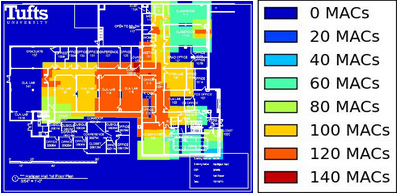
\includegraphics[width=0.5\textwidth]{APContour}
    \caption{First Floor of Halligan Visible Unique MAC Addresses}
\end{figure}


\begin{figure}[h!]
  \centering
    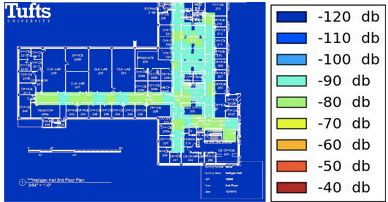
\includegraphics[width=0.5\textwidth]{dbContour}
   \caption{Second Floor of Halligan Median RSS Contour Map}
\end{figure}

Figure 1 examines the MAC addresses visible on the first floor of Halligan, while Figure 2 examines the median RSS values on the second floor of Halligan.

\subsection{Fingerprint Logging Methodology}

\begin{figure}[h!] 
  \centering
    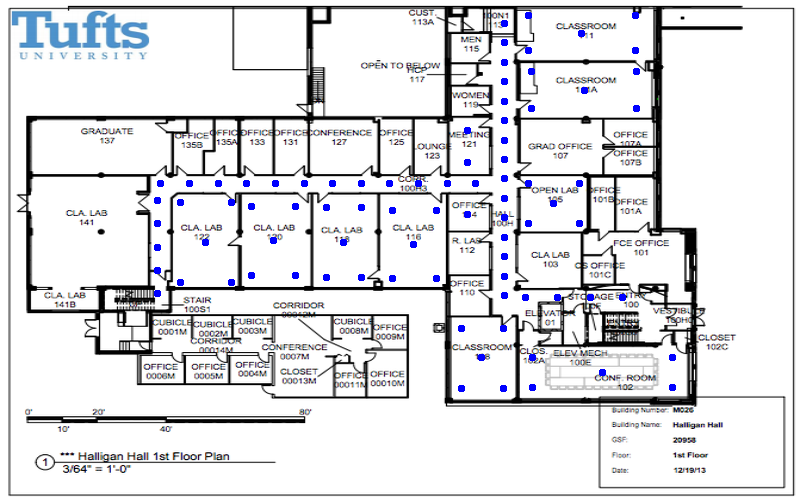
\includegraphics[width=0.5\textwidth]{firstFloor.png}
    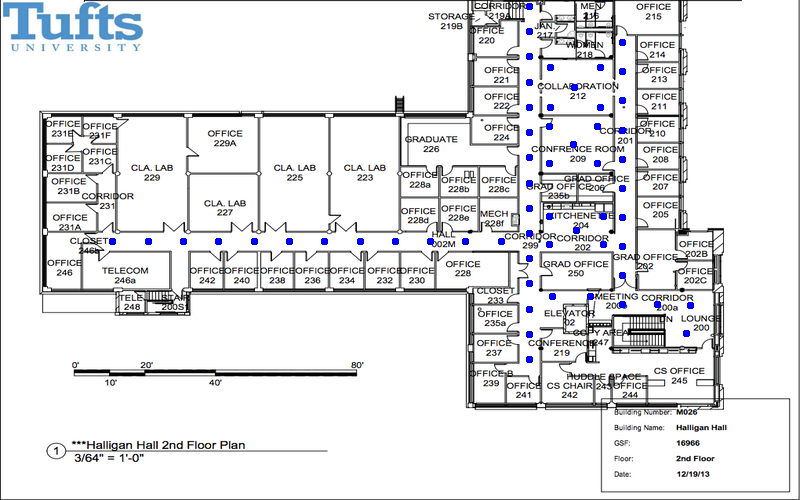
\includegraphics[width=0.5\textwidth]{secondFloor.png}
     \caption{Mapped Positions in Halligan}
\end{figure}

To build the FP database, the average of thirty RSS scans is logged for each position, indicated in Figure 3. The positions in Figure 3 were determined manually through an examination of the floor plans and knowledge of the facility's accessibility. Each recording was stored as four values: a MAC address, an RSS value, a standard deviation, and an association with a location on a map. The recordings were taken at positions estimated with reference to the points in Figure 3.\\
\indent In deciding the number of scans, we considered three factors: time, RSS precision, and MAC address coverage. We tested a sample of scan values between one and one hundred using a single WD. The average Euclidean distance between each of the scans was under 1 dB when using E (discussed in section II.ii.A). Given the similarity of RSS values, we decided to focus on the remaining two factors: time and MAC coverage. \\
\vspace{5mm}\\
\resizebox{\columnwidth}{!}{%
\begin{tabular}{|c|c|c|c|c|c|}
\hline
Scans (1.5s/scan) & 2 & 10 & \textbf{30} & 60 & 100 \\
\hline
Time(Hours )               & 0.24   & 1.2     & \textbf{3.5}     & 7.0      & 12\\
\hline
\end{tabular}
}
\begin{center}
Table 1
\end{center}

\indent Increasing the number of scans improves results, but involves a time tradeoff, as scanning is the most time-consuming part of site survey. With regards to runtime, different WDs had dramatically different scan times, ranging from 0.20 to 2.0 seconds. Table 1 lists the approximate time to record a floor for each number of scans, assuming the worst-case scan time. The number of locations on each floor was based on the average number of locations facing one direction on the two floors of Halligan Hall.\\
\vspace{5mm}\\
\resizebox{\columnwidth}{!}{%
\begin{tabular}{|c|c|c|c|c|c|}
\hline
MAC Coverage(\%) & 2 Scans & 10 Scans & \textbf{30 Scans} & 60 Scans & 100 Scans \\
\hline
Trial 1                & 85.3    & 91.2     & \textbf{96.1}     & 100      & 100       \\
\hline
Trial 2                & 88.7    & 90.3     & \textbf{96.8}     & 100      & 100       \\
\hline
Trial 3                & 74.4    & 79.5     & \textbf{89.2}     & 97.6     & 100       \\
\hline
Trial 4                & 59.6    & 84.3     & \textbf{95.5}     & 97.8     & 100       \\
\hline
Average                & 77.0    & 86.3     & \textbf{94.4}     & 98.9     & 100          \\
\hline
\end{tabular}
}
\begin{center}
Table 2
\end{center}

\indent We chose a number of scans for site surveying which balanced sufficient RSS precision against worst-case device runtime. Given the similarity of MAC coverage, as shown in Table 2, for 30 scans and 100 scans and the runtime implications of each, we opted for 30 scans.\\
\indent When recording the FP database, four devices were utilized: the HTC One m7 (Wi-Fi: IEEE 802.11 a/ac/b/g/n), LG Nexus 4  (Wi-Fi: IEEE 802.11 b/g/n), Samsung Galaxy S3 (Wi-Fi: Wi-Fi 802.11 a/b/g/n), and the Samsung Galaxy Nexus(Wi-Fi: IEEE 802.11 a/b/g/n). The average distance between each phone's recording of the same physical location was 6.3 dB. This value is notably high compared to an average distance of 1.7 dB between four surveys made using the same phone. Though detrimental to our position finder's accuracy, the decision to map with multiple devices reflects our desire to build a device-agnostic system. Further, supporting all device types significantly sped up the mapping process, as parallel mapping was possible.\\
\indent A final consideration was the direction of the recording device. Direction has been shown to have an effect on measurements [1]. We found an average distance of 4.0 dB between four surveys made with the same WD in the same position, recorded at 90 degree angles from each other. We decided to map facing a single direction, as this reduced mapping time by a factor of four. Our implementation does, however, support mapping with direction for applications requiring higher accuracy.\\
\indent The set of FPs collected during mapping is used as data for our positioning algorithm. Upon receiving a positioning request containing FP A, the algorithm compares A with each FP in the mapped set, using the FPs most similar to A to estimate A's position on the map.

\section{Positioning Algorithms}
Many classifiers are suitable for determining the location of an unknown point given an RSS Fingerprint map [2][3]. In our implementation, we use the deterministic Weighted K-Nearest Neighbor (WKNN) method to perform position estimation. In this section, we discuss the WKNN method and propose several distance metrics to improve its performance. 
\subsection{Weighted K-Nearest Neighbor}
\indent Consider a set S of FPs  where N=[$n_1$, $n_2$, ..., $n_K$] is the set of K FPs from S nearest to some other point $\rho$ by distance metric $\sigma$, which quantifies distance as a function of RSS. The estimated location $\rho$ is calculated as:
\begin{equation}
\label{wknn}
\hat{\rho} = \sum\limits_{i=1}^{K}\frac{\omega_i}{\omega_{total}}\rho'_i, \quad w_i = \sigma(n_i, \rho)^{-1}
\end{equation}
where $\omega_i$ is the weight of $n_i$, $\rho'_i$ is the position corresponding to $n_i$, $\omega_{total}$ is the sum of the weights of all FPs in N, and $\sigma(n_i, \rho)$ is the signal distance between $n_i$ and $\rho$ using distance metric $\sigma$. The K-Nearest Neighbor (KNN) method uses equal weights for all fingerprints in N [5]. The specific distance metrics used in our implementation are discussed in the next section. We use WKNN because it has been shown to have a higher accuracy than merely the Nearest Neighbor (NN) method, K = 1, yielding best results with K values of 3 or 4 [5]. 

\subsection{Distance Metrics}
WKNN is a very flexible classifier, and can incorporate a variety of distance metrics. In this section, we discuss the four distance metrics we used to quantify difference between two RSS measurements: Euclidean distance ($\sigma_E$), penalty-weighted Euclidean distance ($\sigma_{E'}$), inverse Jaccard coefficient ($\sigma_{J^{-1}}$), and a linear combination of $\sigma_{E'}$ and $\sigma_{J^{-1}}$ ($\sigma_{E' + J^{-1}}$). For consistency in our definitions, we here define two FPs A and B with RSS vectors a=[$a_1$, $a_2$, ... , $a_m$] and b=[$b_1$, $b_2$, ... , $b_n$], respectively. 

\subsubsection{Euclidean Distance ($\sigma_E$)}

\indent In the ideal case where the sets of MAC addresses seen by A and B are identical, the Euclidean distance between A and B is calculated as:
\begin{equation}
\label{euclidean_ideal}
\sigma_{E_{ideal}}(A, B) = (\sum\limits_{i}|a_i - b_i|^2)^\frac{1}{2}
\end{equation}
where the MAC address of $a_i$ corresponds to that of $b_i$. However, in a realistic environment, there will often be several MAC addresses seen by A and not by B, and vice-versa. One proposed means of handling these mismatches is to assign a threshold value equal to the lowest recorded RSS measurement in the FP database to missing RSS measurements [9]. By this definition, the Euclidean distance between A and B is calculated as:
\begin{equation}
\label{euclidean}
\resizebox{0.45\textwidth}{!}{$\sigma_{E}(A, B)=(\sum\limits_{i}|a_i-b_i|^2+\sum\limits_{j, b_j\notin b}|a_j-I_{min}|^2+\sum\limits_{k, a_j\notin a}|I_{min}-b_k|^2)^\frac{1}{2}$}
\end{equation}
where $I_{min}$ is the lowest recorded RSS measurement in the FP database. In most cases, this has the desired effect of increasing the distance between two locations with non-matching MAC addresses.

\subsubsection{Penalty-Weighted Euclidean Distance ($\sigma_{E'}$)}
\indent One potential issue with the aforementioned means of handling mismatches is that it may result in false matches, in the case where A sees a MAC address with a very low RSS value and B does not see that MAC address. To address this issue, we propose the penalty-weighted Euclidean distance, defined as follows:
\begin{equation} \label{eq1}
\begin{split}
\sigma_{E}(A, B) & = (\sum\limits_{i}|a_i-b_i|^2 \\
			& +  \alpha*\sum\limits_{j, b_j\notin b}|a_j-I_{min}|^2 \\
			& + \alpha*\sum\limits_{k, a_j\notin a}|I_{min}-b_k|^2)^\frac{1}{2}
\end{split}
\end{equation}

where $\alpha$ is a constant value. By introducing a new coefficient, we enable our algorithm to assign a different weight to mismatching MAC addresses.  Through iterative testing, we determined the best value of $\alpha$ to be 0.25. This allows for an increased distance for locations with non-matching MAC addresses but limits the effect of false RSS matches.
	
\subsubsection{Inverse Jaccard Coefficient ($\sigma_{J^{-1}}$)}
\indent The Jaccard coefficient is equal to the number of elements in the intersection divided by the number of elements in the union [7]. The larger the Jaccard coefficient, the greater the similarity between the two sets. We use the inverse Jaccard coefficient with our implementation of WKNN, as small values indicate similarity within the WKNN algorithm. The inverse Jaccard coefficient is calculated as:  
\begin{equation}
\label{jaccard}
\sigma_{J^{-1}}(A, B) = (\frac{|a\cap b|}{a\cup b})^{-1}
\end{equation}
The inverse Jaccard coefficient is small when the MAC addresses have high overlap, which indicates similarity within the WKNN algorithm. As this only examines the MAC addresses, this is a quick yet coarse method to determine distances between locations.

\subsubsection{Linear Combination of $\sigma_{E'}$ and $\sigma_{J^{-1}}$ ($\sigma_{E' + J^{-1}}$)}
\indent Since the penalty-weighted Euclidean distance metric and the inverse Jaccard coefficient both reveal valuable information about the difference between RSS vectors, we propose a new distance metric that is the linear combination of these two measures, defined as follows:
\begin{equation}
\label{combined}
\sigma_{E'+J^{-1}}(A, B) = \beta_1*\sigma_{E'}(A, B)+\beta_2*\sigma_{J^{-1}}(A, B)
\end{equation}
where $\beta_1$ and $\beta_2$ are constants. Through iterative testing, we determined the best values of $\beta_1$ and $\beta_2$ to be 1.0 and 0.45, respectively. This result utilizes the effectiveness of the penalty-weighted Euclidean distance metric at detecting differences in RSS values for common MAC addresses, as well as the ability of the inverse Jaccard metric to penalize unique MAC addresses.

\section{Map-Aware Algorithm Refinement Techniques}

In addition to the distance metrics used in our WKNN algorithm, we made several changes to our map structure and algorithm execution that improved the performance of our position finder. 

\subsection{Density-Penalizing Neighbor Weighting}
\indent A neighbor factor was added to improve accuracy when locating positions in sparsely mapped buildings. This factor improved accuracy when locating points in corners and near the edges of the mapped areas. We define the neighbor factor $W_d$ for some point $d$, as:
\begin{equation}
\label{density}
\begin{split}
W_d=\phi*\sum\limits_{i}F(d,di)\\
F(d,di)=\{\begin{array}{lr}
       1: &  \sigma_E(d, d_i) < \Gamma \\
       0: &  otherwise
\end{array}
\end{split}
\end{equation}
where $\phi$ is a constant, $d_i$ is the $i^{th}$ fingerprint in the database, and $\Gamma$ is the neighbor threshold. Through iterative testing, we determined the optimal value of $\phi$ to be 0.08 and $\Gamma$ to be 20 meters. The minimum neighbor count is always one, as a point is always its own neighbor; this ensures a non-zero value in all cases. This factor increases the importance of points with low neighbor counts, helping improve accuracy in areas that are sparsely mapped. 

\subsubsection*{Floor Detection Pre-Processing}
\indent Before running WKNN with a more complex distance metric, we first run it using only the inverse Jaccard coefficient in order to determine the floor of our test point. We do this because calculating the inverse Jaccard coefficient between two sets of MAC addresses does not require any calculations involving signal strength, so it does not take as much computational time as calculating Euclidean distance. Once we have determined the floor of our test point, we find its coordinates by running WKNN with distance $\sigma_C$ (defined in the next section), only iterating over fingerprints in the database on the correct floor. While this change does not yield significant time improvements given our test environment that only contains two floors, its benefits become more evident in an environment with several floors and buildings.

\subsection{Composite Distance Metric $\sigma_C$}
\indent Our WKNN measures distance as a linear combination of Euclidean distance with penalty, $\sigma_{E'}$,  the inverse Jaccard distance $\sigma_{J^{-1}}$, and the neighbor count weighting, $W$,  given as follows:
\begin{equation}
\label{composite}
\sigma_C(A, B)=\beta_1*\sigma_{E'}(A, B)+\beta_2*\sigma_{J^{-1}}(A, B)+W_B
\end{equation}
where $\beta_1$ and $\beta_2$ are constants. This metric allows for a combination of comparing the similarity of signal strengths through the penalty-weighted Euclidean distance, comparing the similarity of seen MAC addresses through the inverse Jaccard coefficient, and an additional weighting with the neighbor factor. This composite distance metric is evaluated in the next section and compared to each of the component distant metrics.

\section{Performance}

Ultimately, our positioning application has an average error of 2.66m meeting the requirements of most commercial applications. We break our analysis into three sections. First, we discuss our testing methodology. Second, we compare our four distance metrics: Euclidean distance ( $\sigma$), penalty-weighted Euclidean distance ( $\sigma_{E'}$), inverse Jaccard coefficient ($\sigma_{J^{-1}}$), and a linear combination of$\sigma_{E'}$ and $\sigma_{J^{-1}}$ ($\sigma_{E' + J^{-1}}$). Finally, we analyze our map-aware algorithm refinements: Floor Detection Preprocessing and Density-Penalizing Neighbor Weighting.

\subsection{Testing Methodology}
We recorded a set of points for the purpose of fine-tuning our coefficients, called the coefficient training set, as well as a second set of points for performance testing, called the testing set. Both sets contain points randomly generated by the Mitchell's Best Candidate II algorithm, which efficiently creates a Poisson Distribution of points within the mapped regions [6] displayed in Figure 4. All FPs in the testing set were recorded using the HTC One m7. 

\begin{figure}[h!]
  \centering
    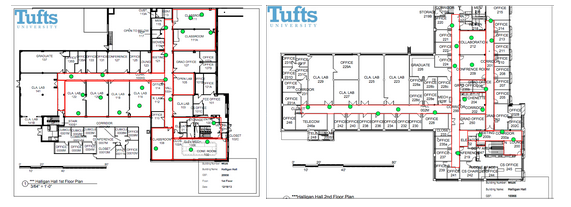
\includegraphics[width=0.5\textwidth]{testpoints}
   \caption{Test points on Halligan Floor 1 (left) and Floor 2 (right); red boxes indicate accessible regions, and green dots indicate test points}
\end{figure}

The accuracy of our positioning algorithm is dependent on the number of scans the WD makes, as shown in Figure 5. Increasing the number of scans beyond five does not significantly improve the performance of our algorithm; therefore, we chose to test our positioning application against FPs gathered with five scans.

\begin{figure}[h!]
  \centering
    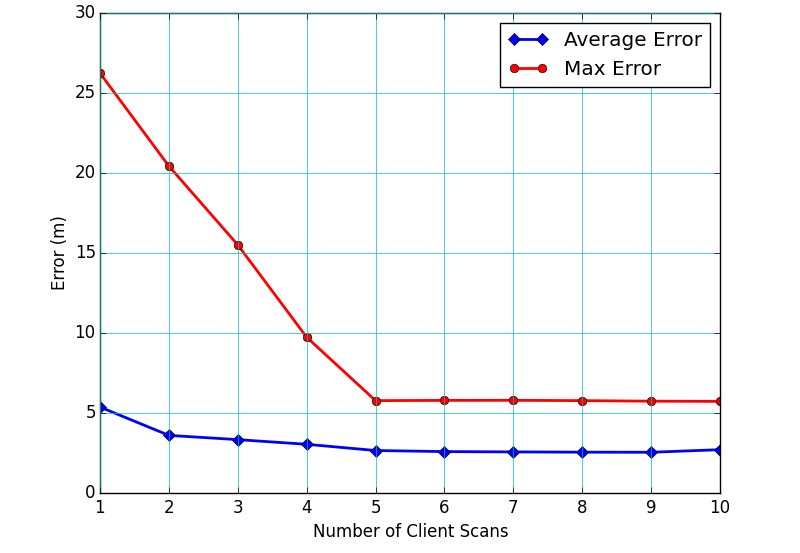
\includegraphics[width=0.5\textwidth]{pull_errors.png}
   \caption{Accuracy of composite distance metric for various numbers of positioning scans}
\end{figure}

\subsection{Distance Metric Comparisons}
We tested our WKNN algorithm iteratively with the coefficient training set and found the algorithm had the best performance when K = 3. Figure 6 shows the observed accuracy of our WKNN algorithm using four different distance metrics. As the graph shows, the standard Euclidean distance metric performs significantly better than the inverse Jaccard coefficient, yielding average errors of 3.56m and 4.75m, respectively. Using the penalty-Weighted Euclidean Distance reduces the error to 2.87m. A linear combination of the two metrics only improves the performance slightly, bringing the error to 2.78m. However, the linear combination reduces the maximum error to 9.70m, which is 21.1\% smaller than that of the Penalty-Weighted Euclidean distance metric.

\begin{figure}[h!]
  \centering
    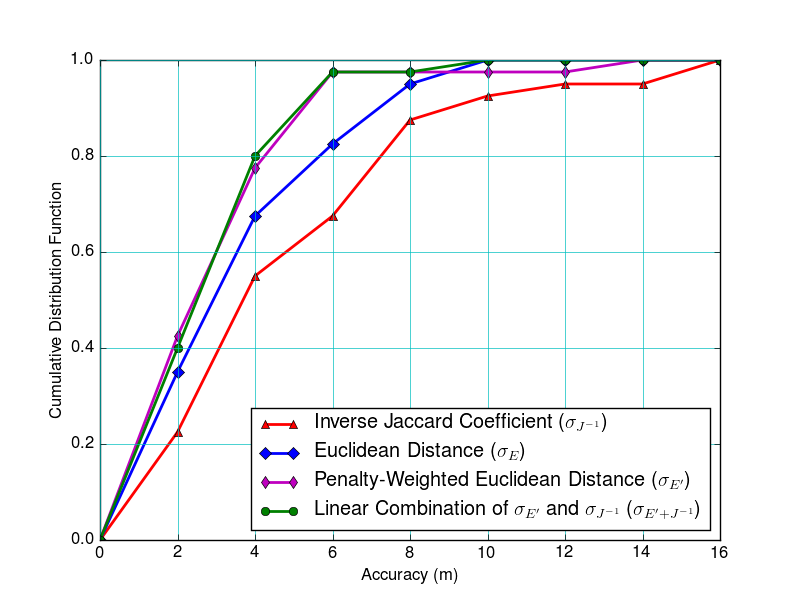
\includegraphics[width=0.5\textwidth]{distance_comparison.png}
    \caption{CDF of positioning accuracy for various WKNN distance metrics (K=3)}
\end{figure}


\subsection{Map-Aware Algorithm Refinement}

We add our Neighbor-Weighting as a parameter to our composite distance metric ($\sigma_C$). Overall, Neighbor-Weighting decreases the average error from 2.78m to 2.66m. For points with less than 5m error, Neighbor-Weighting increases the average error by 0.15m. However, the technique reduces the maximum error by 40.5\%, from 9.70m to 5.77m, and the average error of points with more than a 5m error by 50.1\%, from 7.12m to 3.55m. We consider this slight increase in average error well worth the dramatic reduction in maximum error.\\		
\indent Figure 7 shows the effect of our floor detection preprocessing technique on runtime. For this calculation, we assume 100 fingerprints per floor. This preprocessing does not improve runtime results in our testing environment, but our simulation indicates that this technique would reduce positioning time by 39.1\%, from 6.89 seconds to 4.20 seconds, for a system with 100 floors.This time reduction results from the reduced number of penalty-weighted Euclidean distance calculations required.

\begin{figure}[h!]
  \centering
    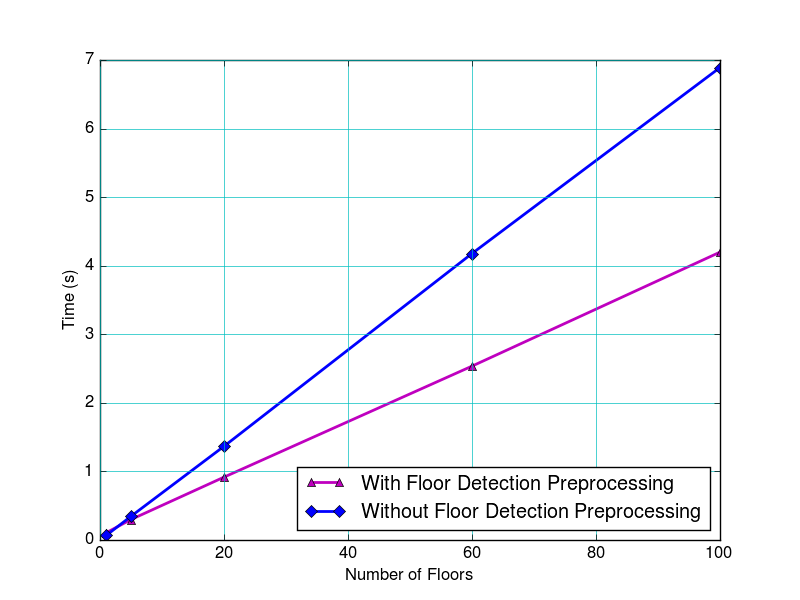
\includegraphics[width=0.5\textwidth]{time_comparison.png}
   \caption{Effect of floor detection preprocessing technique on positioning time}
\end{figure}

This performance improvement would be extremely significant in a large-scale commercial application.

\section{Discussion}
\indent Our positioning application has runtime and accuracy similar to other fingerprint-based systems [10]. Although there are fingerprinting positioning systems with higher accuracy, many utilize application-specific hardware, whereas our application operates with  consumer hardware and no assumed site information.\\
\indent One specific example is the Microsoft RADAR system, which utilizes a basic KNN algorithm with RF signals. Although several systems have come out since RADAR that are improvements, the system achieved similar average error distances, 3 - 5 meters, while operating on a single, highly arranged floor, with the three base stations placed by the developing team, and a single set of hardware utilized. Our system demonstrates that this level of accuracy can be realized with consumer hardware in a commercial-like setting. Similar to how RADAR was able to utilize techniques such as continual user tracking, as well as multiple radio maps for different environments such as time of day [12], we believe our implementation could be improved with these methods while still utilizing a device agnostic system.\\
\indent A system proposed in 2013 uses improved double-peak Gaussian distributions and a probabilistic approach to determine position. This approach used a single device for mapping, and reports an average error of 1.5 meters [13]. While this is a significantly higher accuracy, the techniques used could be incorporated into our positioning application to achieve a similar accuracy.\\ 
\indent Beyond increasing scan numbers, several other methods and data could be incorporated to further improve our system accuracy, including direction in site-survey, WD inertia, and prior knowledge of the site. These options are left as future work.



\section{Conclusion}
Our positioning system addressing many of the obstacles to widespread indoor positioning system implementation. The positioning system we implement is device-agnostic, able to serve multiple users, places no requirements on the site, and has an average error of 2.66m, satisfying the requirements of most applications. We propose two metrics for use with the WKNN algorithm, Density-Penalizing Neighbor Weighting and Penalty-Weighted Euclidean Distance, as well an algorithm modification for improved scalability, Floor Detection Preprocessing. Future work could integrate other algorithm improvement techniques, such as Double Gaussian Distribution processing, and could investigate the performance of user-feedback in the mapping process.


\section*{Acknowledgment}
We would like to thank our research advisor Professor Mai Vu of the Tufts University Electrical Engineering and Computer Science department for providing invaluable guidance and feedback. We would also like to thank Professor Chris Gregg of Tufts University for his advice and encouragement.


%----------------------------------------------------------------------------------------
%	REFERENCE LIST
%----------------------------------------------------------------------------------------

\begin{thebibliography}{99}

\bibitem{1} Sayed, Ali H., Alireza Tarighat, and Nima Khajehnouri.,
"Challenges Faced in Developing Techniques for Accurate Wireless Location Information."
\emph{IEEE Signal Processing Magazine. IEEE, 1}, July 2005. Web. 11 Mar. 2015.
 
\bibitem{2} Sayed, Ali H., Alireza Tarighat, and Nima Khajehnouri.,
"Performance Comparison of Indoor Positioning Techniques Based on Location Fingerprinting in Wireless Networks."
\emph{IEEE Xplore}, 1 Jan. 2005. Web. 11 Mar. 2015. 
 
\bibitem{3} Chaudhuri, K., D. Sanghi, and P. Bhagwat. ,
"Location Determination of a Mobile Device Using IEEE 802.11b Access Point Signals."
\emph{IEEE Xplore. IEEE}, 16 Mar. 2003. Web. 11 Mar. 2015.

\bibitem{4} Lakmali, B.D.S., and Dias, D. ,
"Database Correlation for GSM Location in Outdoor and Indoor Environments."
\emph{Information and Automation for Sustainability, 2008. ICIAFS 2008. 4th International Conference on, vol., no., pp.42,47,}, 12-14 Dec. 2008.
 
\bibitem{5} Kokkinis, Akis; Raspopoulos, Marios; Kanaris, Loizos; Liotta, Antonio; Stavrou, Stavros,
"Map-aided fingerprint-based indoor positioning,"
\emph{Personal Indoor and Mobile Radio Communications (PIMRC), 2013 IEEE 24th International Symposium on}, vol., no., pp.270,274, 8-11 Sept. 2013.

\bibitem{6} Dunbar, Daniel, and Greg Humphreys.,
"A Spatial Data Structure for Fast Poisson-Disk Sample Generation."
\emph{www.cs.virginia.edu. University of Virginia},  1 Jan. 2006. Web. 11 Mar. 2015. 

\bibitem{7} Machaj, Juraj, Peter Brida, and Robert Piche.,
"Rank Based Fingerprinting Algorithm for Indoor Positioning."
\emph{ International Conference on Indoor Positioning and Indoor Navigation IPIN, Guimaraes, Portugal},  21-23 September 2011. Web. 12 Mar. 2015.

\bibitem{8} Fielding, R.,
"Architectural Styles and the Design of Network-based Software Architectures."
\emph{ (Unpublished Doctoral dissertation). University of California, Irvine.}, 200

\bibitem{9} Kemppi, P.; Nousiainen, S.
"Database Correlation Method for Multi-System Positioning,"
\emph{Vehicular Technology Conference, 2006. VTC 2006-Spring. IEEE 63rd },  vol.2, no., pp.866,870, 7-10 May 2006.

\bibitem{10} Hui Liu, Houshang Darabi, Pat Banerjee, and Jing Li.,
"Survey of Wireless Indoor Positioning Techniques and Systems,"
\emph{ (Systems, Man, and Cybernetics, Part C: Applications and Reviews, IEEE Transactions on.}, vol.37, no.6, pp.1067,1080, Nov. 2007 

\bibitem{11} P. Bahl and V. N. Padmanabhan,
RADAR: An in-building RF-based user location and tracking system,
\emph{in Proc. IEEE INFOCOM}, 2000, Mar., vol. 2, pp. 775-784.

\bibitem{12} P. Bahl and V. N. Padmanabhan,
Enhancements to the RADAR user location and tracking system,
\emph{Microsoft Corp., Tech. Rep. MSR-TR- 2000,12}, Feb. 2000.

\bibitem{13} Chen, Lina, Binghao Li, Kai Zhao, Chris Rizos, and Zhengqi Zheng,
"An Improved Algorithm to Generate a Wi-Fi Fingerprint Database for Indoor Positioning."
\emph{Sensors (Basel, Switzerland). Molecular Diversity Preservation International (MDPI)}, 8 Aug. 2013. Web. 03 Apr. 2015.


\end{thebibliography}



% that's all folks
\end{document}


